%%%%%%%%%%%%%%%%%%%%%%%%
% $Autor: MansourAhmadyPhoulady, RanjeetsingTawar, HemanthPrabhakaran$
% $Pfad: Car_Licence_Plate_Identification_with_a_JetsonNano$
% $Version: 4.0.0 $
%
% !TeX encoding = utf8
%
%%%%%%%%%%%%%%%%%%%%%%%%

\chapter{Development Environment and Software Description}

\section{Integrated Development Environment (IDE)}

An Integrated Development Environment (IDE) serves as a comprehensive platform designed to streamline the software development process. By integrating essential tools such as a code editor, debugger, and compiler into a unified interface, an IDE simplifies the development workflow. It enhances productivity through features like syntax highlighting, code completion, and real-time code analysis, reducing the likelihood of errors and expediting debugging. Additionally, most modern IDEs provide project management capabilities, version control integration, and support for team collaboration, making them indispensable for both individual and collaborative projects.

\subsection{Features of IDEs}

Key features commonly found in IDEs include:
\begin{itemize}
	\item \textbf{Code Editor:} Provides syntax highlighting, indentation, and real-time error detection.
	\item \textbf{Debugger:} Offers tools for setting breakpoints, stepping through code, and analyzing program execution.
	\item \textbf{Compiler/Interpreter:} Facilitates code compilation or interpretation for immediate execution and testing.
	\item \textbf{Version Control Integration:} Enables seamless interaction with Git, SVN, or other version control systems for tracking changes and collaboration.
	\item \textbf{Project Management Tools:} Helps organize files, directories, and configurations within a project.
	\item \textbf{Extensions and Plugins:} Allows customization and expansion of functionality to cater to specific development needs.
\end{itemize}

\subsection{Popular IDEs}

The following are some of the widely used IDEs, each offering unique features tailored to different programming needs:

\begin{enumerate}
	\item \textbf{PyCharm:} 
	PyCharm is a robust IDE specifically designed for Python development. It is renowned for features such as intelligent code completion, advanced debugging, refactoring tools, and support for web frameworks like Django and Flask. Its professional edition includes integrated database tools, making it ideal for data-centric applications.
	
	\item \textbf{Visual Studio Code:} 
	Visual Studio Code, or VS Code, is a lightweight yet powerful cross-platform IDE. It supports multiple programming languages through extensions and offers features like built-in Git integration, debugging capabilities, and customizable themes. Its versatility makes it a popular choice among developers across various domains.
	
	\item \textbf{Jupyter Notebook:} 
	Jupyter Notebook is a web-based IDE that excels in interactive computing. It allows developers to write and execute code in a cell-based environment, making it particularly well-suited for data science, machine learning, and data analysis projects. Its ability to combine code, visualizations, and markdown in a single document enhances collaboration and presentation.
	
	\item \textbf{Spyder:} 
	Spyder is an open-source IDE geared toward scientific computing and data analysis. It integrates seamlessly with libraries such as NumPy, SciPy, and Matplotlib, and includes features like variable explorers and inline plotting, making it a preferred choice for researchers and scientists.
	
	\item \textbf{Eclipse:} 
	Eclipse is a versatile IDE primarily used for Java development but supports other languages through plugins. It features extensive debugging tools, project management support, and integration with build automation tools like Maven and Gradle.
	
	\item \textbf{IntelliJ IDEA:} 
	IntelliJ IDEA is a powerful IDE for Java and Kotlin development. It offers advanced features such as smart code completion, deep static code analysis, and tools for managing complex codebases. Its robust ecosystem supports a wide range of frameworks and languages.
\end{enumerate}

\subsection{Comparison of IDEs}

Each IDE has its strengths, making it suitable for different use cases. For instance:
\begin{itemize}
	\item \textbf{PyCharm:} Ideal for Python developers who require advanced debugging and web development support.
	\item \textbf{VS Code:} Versatile for developers working with multiple languages and requiring a lightweight setup.
	\item \textbf{Jupyter Notebook:} Best suited for data scientists and analysts who value interactivity and visualization.
	\item \textbf{Spyder:} Designed for scientific and numerical computing.
	\item \textbf{Eclipse:} Preferred for large-scale Java projects.
	\item \textbf{IntelliJ IDEA:} Optimal for enterprise-level Java and Kotlin development.
\end{itemize}

\subsection{Selected IDE for the Project}

For this project, \textbf{PyCharm} and \textbf{Jupyter Notebook} have been chosen as the primary IDEs due to their complementary features. PyCharm is used for managing the overall project structure, implementing object detection algorithms, and integrating TensorFlow models. Jupyter Notebook, on the other hand, is utilized for interactive data analysis and experimentation, particularly during model training and validation phases. This combination ensures both efficiency and flexibility in the development workflow.




\subsection{PyCharm}
PyCharm is a robust and feature-rich Integrated Development Environment (IDE) specifically designed for Python programming. It provides an extensive set of tools and functionalities that streamline the development workflow, ensuring productivity and efficiency. PyCharm supports a broad spectrum of Python applications, including web development, data science, machine learning, and automation, making it a preferred choice for developers across various domains.

\subsection{PyCharm Main Functions and Sub-functions}

Below is a detailed breakdown of the primary functions in PyCharm and their corresponding subfunctions:

\begin{enumerate}
	\item \textbf{Code Editing}:
	\begin{itemize}
		\item \textbf{Syntax Highlighting:} Differentiates syntax elements using color coding for better readability and easier debugging.
		\item \textbf{Code Completion:} Provides intelligent, context-aware suggestions for completing code based on imports, libraries, and project-specific definitions.
		\item \textbf{Code Formatting:} Automatically adjusts code layout to adhere to PEP-8 standards or customized style guides.
		\item \textbf{Code Navigation:} Facilitates quick access to classes, functions, and methods through navigation shortcuts.
		\item \textbf{Code Snippets:} Offers predefined templates for frequently used code blocks to accelerate development.
	\end{itemize}
	
	\item \textbf{Debugging}:
	\begin{itemize}
		\item \textbf{Breakpoints:} Enables developers to pause execution at specific lines to analyze the program state.
		\item \textbf{Variable Inspection:} Displays the current state and values of variables during runtime.
		\item \textbf{Step-through Debugging:} Allows developers to execute code line-by-line to trace logic errors and bugs.
		\item \textbf{Call Stack Exploration:} Visualizes the sequence of function calls leading to a particular point in the execution.
	\end{itemize}
	
	\item \textbf{Testing}:
	\begin{itemize}
		\item \textbf{Testing Frameworks Integration:} Built-in support for popular testing frameworks like \texttt{pytest}, \texttt{unittest}, and \texttt{doctest}.
		\item \textbf{Test Runner:} Executes test cases and generates detailed reports, highlighting passed, failed, and skipped tests.
		\item \textbf{Code Coverage Analysis:} Measures and visualizes the extent of code covered by test cases.
		\item \textbf{Test Coverage Highlighting:} Displays untested parts of the code directly in the editor.
	\end{itemize}
	
	\item \textbf{Version Control}:
	\begin{itemize}
		\item \textbf{Git Integration:} Seamless interaction with Git, enabling commit, push, pull, and merge operations directly within the IDE.
		\item \textbf{Commit and Update:} Simplifies committing local changes and fetching updates from remote repositories.
		\item \textbf{Branching and Merging:} Provides an intuitive interface for creating, switching, and merging branches.
		\item \textbf{Diff Viewer:} Highlights differences between code versions for easy conflict resolution.
	\end{itemize}
	
	\item \textbf{Web Development}:
	\begin{itemize}
		\item \textbf{Framework Support:} Supports web frameworks like Django, Flask, and FastAPI with dedicated tools for their development.
		\item \textbf{HTML/CSS/JavaScript Support:} Includes syntax highlighting, autocomplete, and inspection for front-end languages.
		\item \textbf{Web Server Integration:} Runs and debugs web applications directly within PyCharm.
		\item \textbf{Template Language Support:} Provides tools for working with Jinja2, Mako, and other template engines.
	\end{itemize}
	
	\item \textbf{Database Tools}:
	\begin{itemize}
		\item \textbf{Database Connectivity:} Establishes connections to databases like PostgreSQL, MySQL, and SQLite for data querying.
		\item \textbf{SQL Editor:} Aids in writing and executing SQL queries with syntax highlighting and autocomplete.
		\item \textbf{Database Explorer:} Allows navigation through database schemas, tables, and records.
	\end{itemize}
	
	\item \textbf{Collaboration}:
	\begin{itemize}
		\item \textbf{Version Control Integration:} Facilitates team collaboration by integrating with Git, GitHub, Bitbucket, and more.
		\item \textbf{Code Review Tools:} Allows reviewing, commenting, and discussing changes made by team members.
		\item \textbf{Remote Development:} Supports development on remote servers through SSH or Docker integration.
	\end{itemize}
\end{enumerate}

\subsection{Importance of Python in the Project}

The methodologies employed in this project heavily rely on Python 3.9, chosen for its versatility and extensive library ecosystem. Python serves a broad spectrum of applications, including:
\begin{itemize}
	\item Development of desktop applications, command-line tools, and games.
	\item Data analysis and scientific computing with libraries like NumPy and Pandas.
	\item Automation of administrative and DevOps tasks.
	\item Machine learning and AI applications using TensorFlow, PyTorch, and scikit-learn.
	\item Web development through frameworks like Django and Flask.
\end{itemize}

\textbf{Prerequisites:} Ensure Python 3.9 is installed on your system before proceeding with the project. This can be done by downloading it from the \href{https://www.python.org/downloads/}{official Python website}.


\section{Installation of Python 3.9}

Installing Python 3.9 is the foundational step for setting up the development environment. Below are the detailed steps for installation:

\begin{enumerate}
	\item \textbf{Download Python:} Visit the official Python website at \url{https://www.python.org/downloads/} and download Python 3.9.6 by clicking the appropriate download link.
	\begin{figure}[h!]
		\centering
		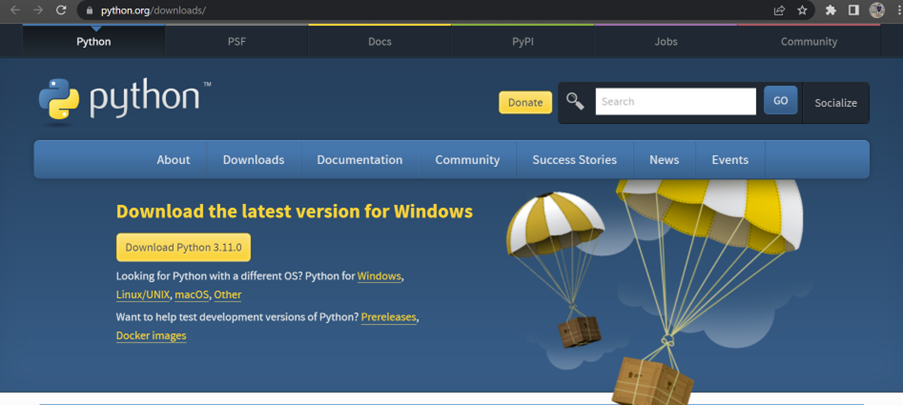
\includegraphics[width=0.8\textwidth]{Images/Python1}
		\caption{Python 3.9.6 Download Page}
	\end{figure}
	
	\item \textbf{Run the Installer:} Open the downloaded file to start the Python setup. A pop-up window for Python 3.9.6 (64-bit) Setup will appear.
	\begin{figure}[h!]
		\centering
		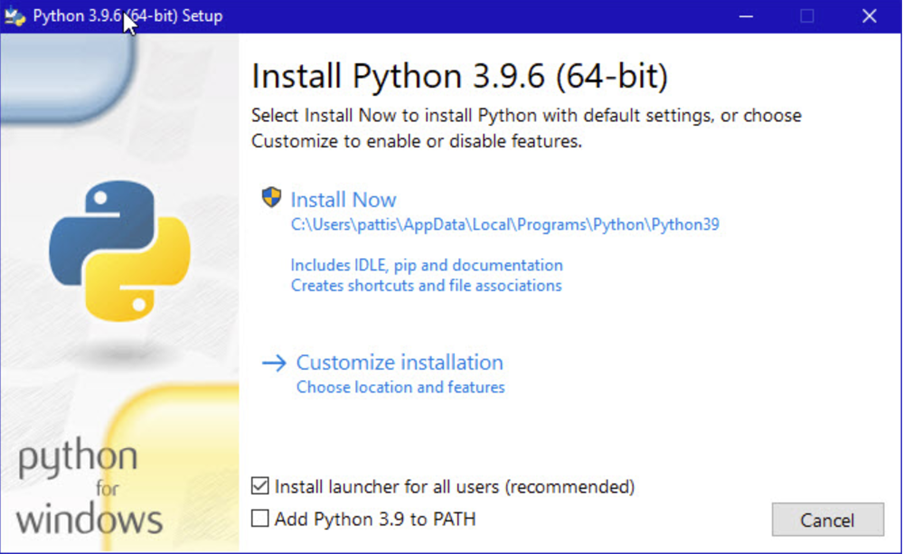
\includegraphics[width=0.8\textwidth]{Images/Python2}
		\caption{Python Setup Window}
	\end{figure}
	
	\item \textbf{Select Installation Options:} Follow the instructions on the setup window. Ensure that the box labeled “Add Python 3.9 to PATH” is checked. This ensures Python is accessible from the command line.
	\begin{figure}[h!]
		\centering
		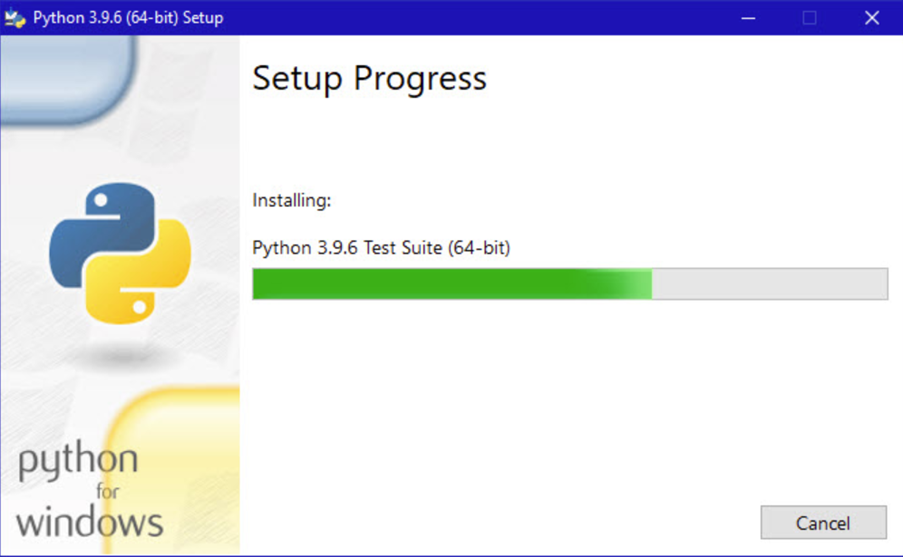
\includegraphics[width=0.8\textwidth]{Images/Python3}
		\caption{Setup Progress Window}
	\end{figure}
	
	\item \textbf{Verify Installation:} After installation, open the Command Prompt (or terminal) and type:
	\begin{lstlisting}[language=bash]
		python --version
	\end{lstlisting}
	This command should display the installed version of Python.
	\begin{figure}[h!]
		\centering
		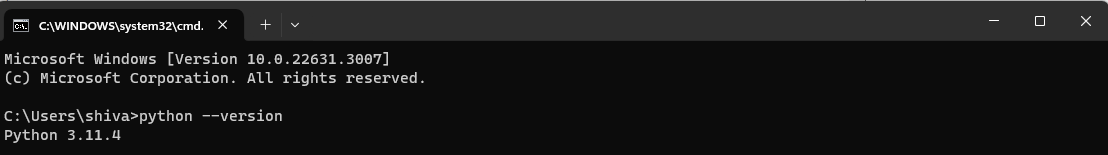
\includegraphics[width=0.7\textwidth]{Images/Python5}
		\caption{Verifying Python Installation}
	\end{figure}
\end{enumerate}

\section{Installation of PyCharm}

PyCharm is a widely-used IDE for Python development. It simplifies the coding process with features such as intelligent code completion, debugging, and virtual environment management. Follow these steps to install PyCharm:

\begin{enumerate}
	\item \textbf{Download PyCharm:} Visit the PyCharm download page at \url{https://www.jetbrains.com/pycharm/download/} and click the “DOWNLOAD” link under the PyCharm Professional Edition.
	\begin{figure}[h!]
		\centering
		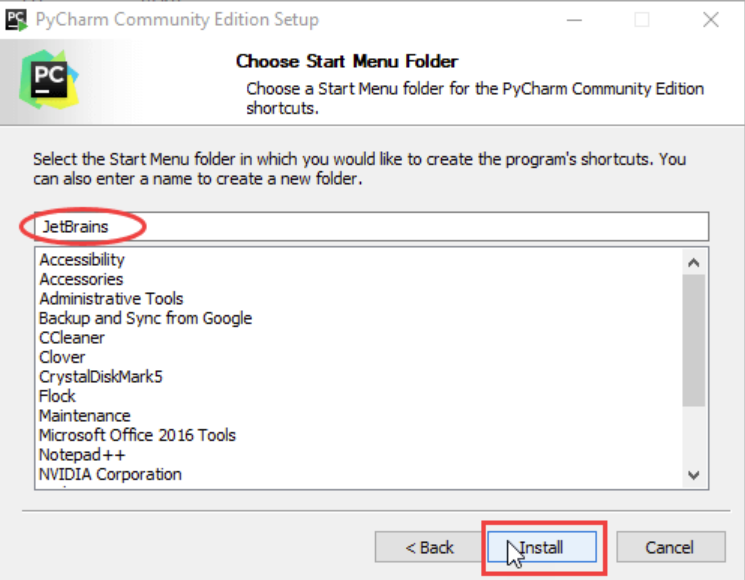
\includegraphics[width=0.8\textwidth]{Images/Pycharm1}
		\caption{Downloading PyCharm Professional Edition}
	\end{figure}
	
	\item \textbf{Complete Installation:} Run the installer and follow the on-screen instructions. Once the installation is complete, check the box to “Run PyCharm Professional Edition” and click “Finish.”
	\begin{figure}[h!]
		\centering
		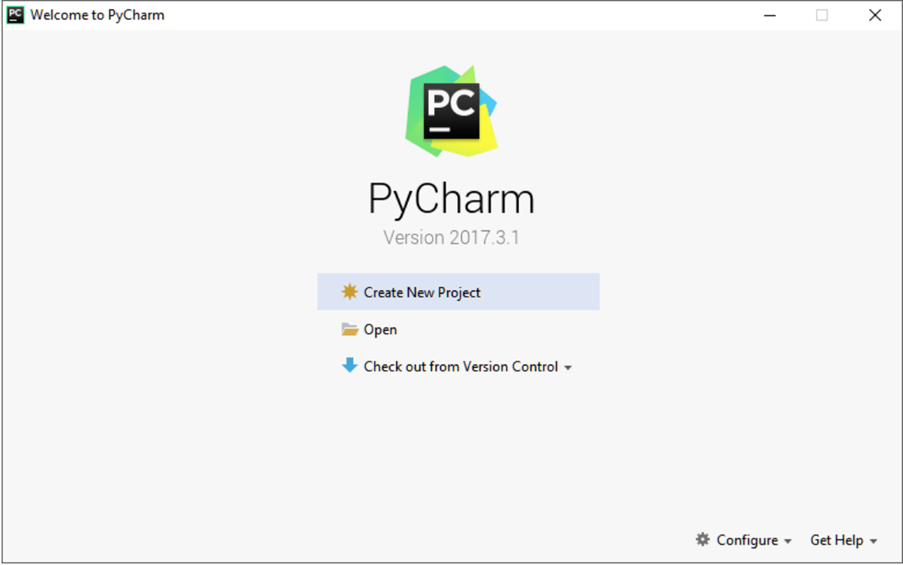
\includegraphics[width=0.8\textwidth]{Images/Pycharm2}
		\caption{PyCharm Startup Window}
	\end{figure}
	
	\item \textbf{Install Required Libraries:} Use PyCharm's integrated terminal or an external terminal to install required libraries. For example:
	\begin{lstlisting}[language=bash]
		pip install -r requirements.txt
	\end{lstlisting}
	\begin{figure}[h!]
		\centering
		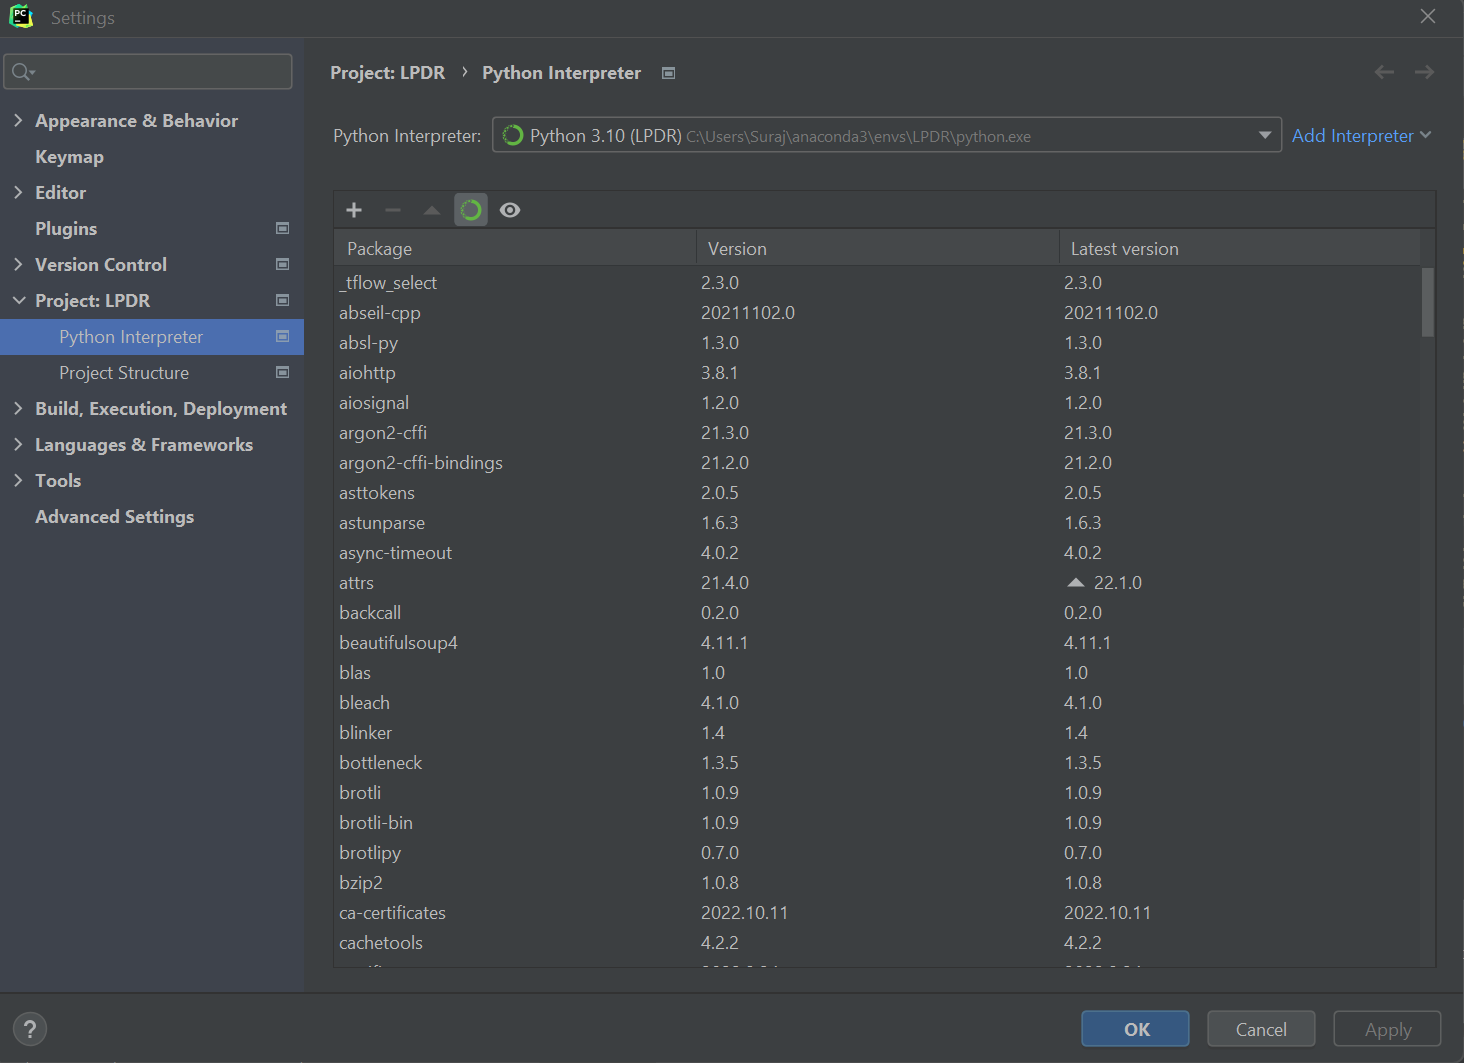
\includegraphics[width=0.8\textwidth]{Images/Pycharm3}
		\caption{Installing Required Libraries in PyCharm}
	\end{figure}
	
	\item \textbf{Start Development:} Import your project directory into PyCharm to begin development. The interface allows for smooth navigation and coding within your environment.
	\begin{figure}[h!]
		\centering
		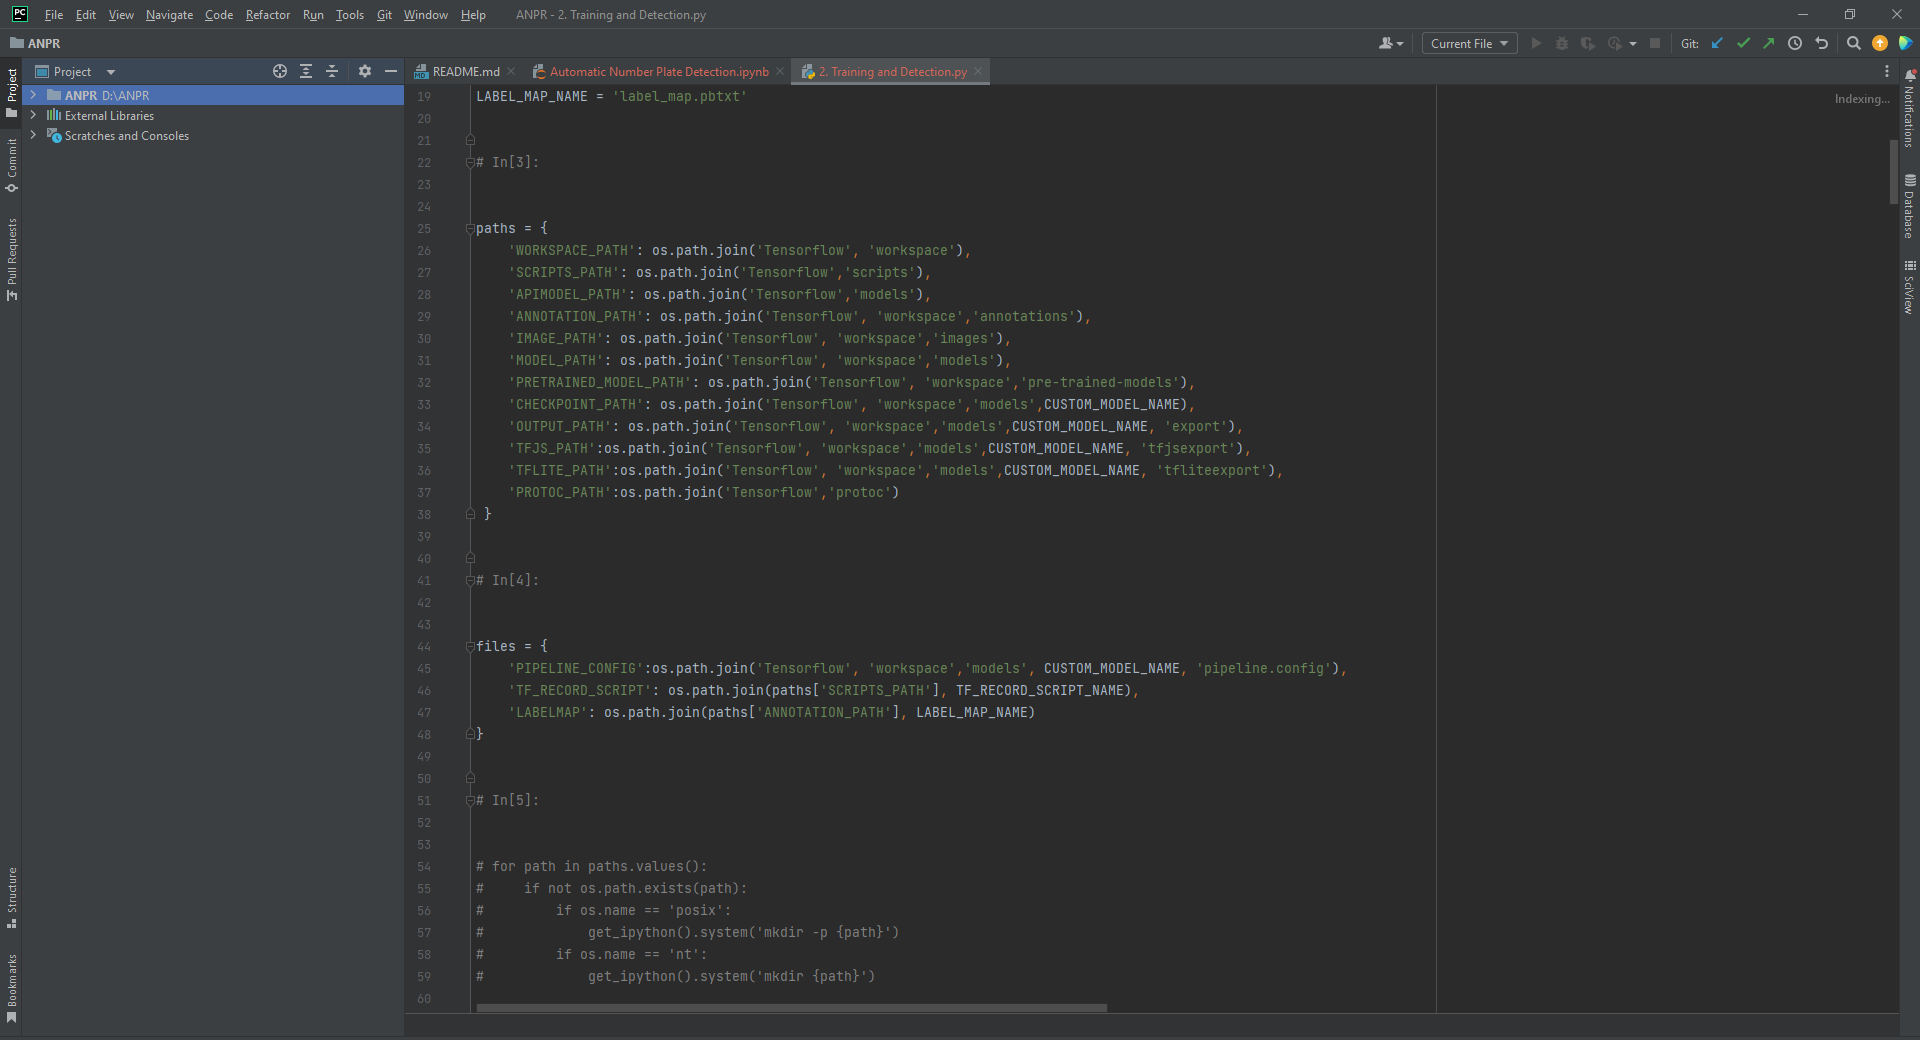
\includegraphics[width=0.8\textwidth]{Images/Pycharm4}
		\caption{Development in PyCharm}
	\end{figure}
\end{enumerate}

\section{Hello World Example}

To verify the installation and start your Python journey, create a simple "Hello, World!" program. Write the following code in PyCharm or any text editor:

\begin{lstlisting}[language=Python]
	print("Hello, World!")
\end{lstlisting}

This code outputs:
\texttt{"Hello, World!"}

\begin{figure}[h!]
	\centering
	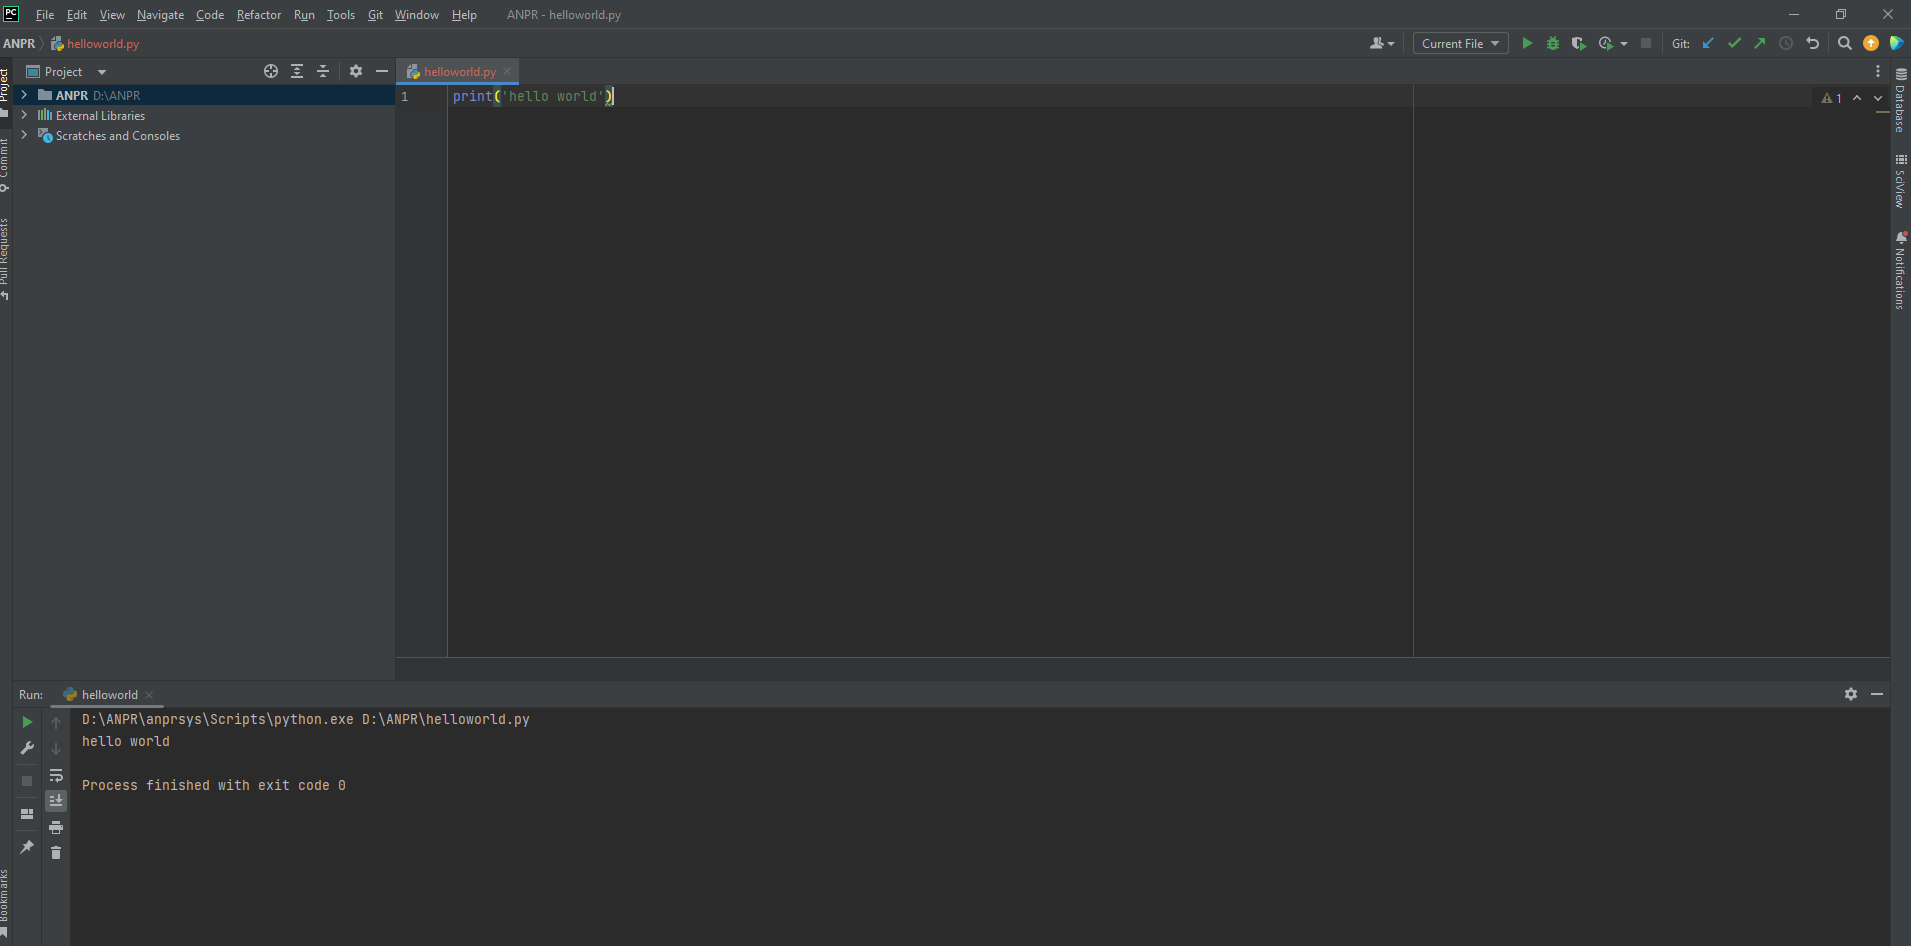
\includegraphics[width=0.7\textwidth]{Images/helloworld}
	\caption{Output of Hello World Program in Python}
	\label{fig:helloworld}
\end{figure}

This basic program validates that Python is properly installed and ready for use. It serves as the traditional first step in exploring a programming language.

\newpage


\section{Overview of the Operating System}

The NVIDIA Jetson family, including the Jetson Nano, is supported by the \textit{JetPack} operating system, a specialized platform designed to optimize performance for machine learning, computer vision, and AI applications. JetPack is based on a Linux kernel, utilizing the Debian Package Management System, which allows developers to harness their existing Linux expertise for seamless interaction with the system. This operating system serves as a comprehensive toolkit for developing cutting-edge AI solutions across the entire Jetson lineup, including the Jetson AGX Xavier and Jetson TX2.

\subsection{Key Features of JetPack}

JetPack integrates a range of powerful modules and frameworks tailored to support high-performance AI applications:

\begin{itemize}
	\item \textbf{CUDA:} A parallel computing platform and application programming interface (API) model that enables developers to utilize NVIDIA GPUs for general-purpose processing tasks.
	\item \textbf{TensorRT:} A high-performance deep learning inference library designed for optimizing and deploying AI models.
	\item \textbf{Computer Vision:} Includes libraries and tools for image processing and object detection tasks.
	\item \textbf{DeepStream SDK:} A toolkit for creating AI-powered video analytics solutions, suitable for applications like surveillance and retail analytics.
\end{itemize}

These modules enable flexible development for a variety of hardware systems, allowing performance to be tailored and scaled based on the specific requirements of an application. By integrating these powerful tools, JetPack provides developers with a versatile platform for deploying advanced AI and deep learning applications on Jetson devices.

\subsection{Development Environment Overview}

The JetPack SDK creates a structured development environment that includes the above modules alongside additional libraries and tools. The figure~\ref{JetsonSDK} illustrates the architecture of the JetPack environment, showcasing its various components and their potential applications. This structure highlights how each module contributes to building scalable, high-performance AI solutions for diverse use cases.

\begin{figure}[h!]
	\centering
	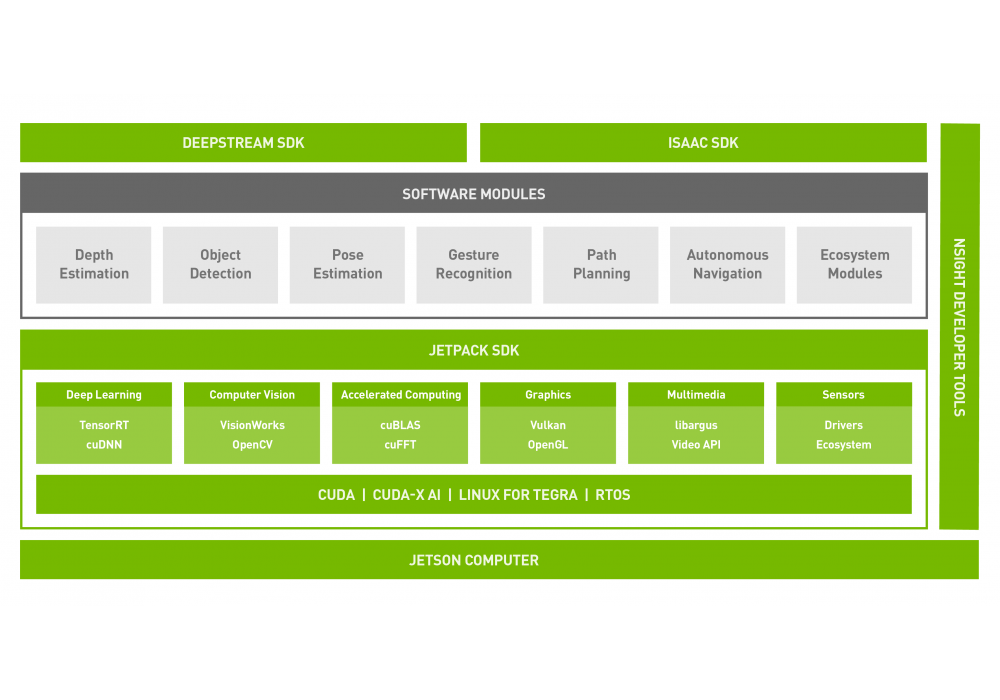
\includegraphics[width=\textwidth]{Images/JetsonNanoSDK}
	\caption{Jetson Nano SDK Development Environment (Source: Heise, 29.11.2019)} 
	\label{JetsonSDK}
\end{figure}

\medskip

By offering a unified operating system and development environment, JetPack empowers developers to leverage the full potential of the Jetson platform for creating innovative, scalable, and efficient AI solutions.




\section{Installing the Operating System}

To set up the Jetson Nano, a properly prepared microSD card is required. This involves downloading the operating system image file from the NVIDIA website and writing it to the microSD card using specialized software. The JetPack operating system is based on Linux and follows a Debian-like file system structure. Once the image is written to the microSD card, it can be inserted into the Jetson Nano for configuration. This section provides a step-by-step guide to installing the operating system.

\subsection{Writing the Operating System to the MicroSD Card}

The operating system image can be downloaded from the official NVIDIA website \cite{JetsonUserManual:2020, JetPackOS:2021}. The image is then written to the microSD card using tools like Etcher, available at \url{https://www.balena.io/etcher/} \cite{JetsonGettingStarted:2019}. 

\subsubsection{Formatting the MicroSD Card}

Before writing the image, the microSD card must be formatted. The procedure for formatting depends on the operating system of the host computer. Below are the steps for formatting the card on Windows:

\begin{enumerate}
	\item \textbf{Download and Install the SD Memory Card Formatter:} 
	Visit the SD Association's official website at \url{https://www.sdcard.org/downloads/formatter/} and download the SD Memory Card Formatter. Install and launch the application.
	
	\item \textbf{Format the MicroSD Card:}
	\begin{itemize}
		\item Insert the microSD card into your computer's SD card reader.
		\item Open the SD Memory Card Formatter. A dialogue window, as shown in Figure~\ref{JetPack:SdFormatierer}, will appear.
		\begin{figure}[h!]
			\centering
			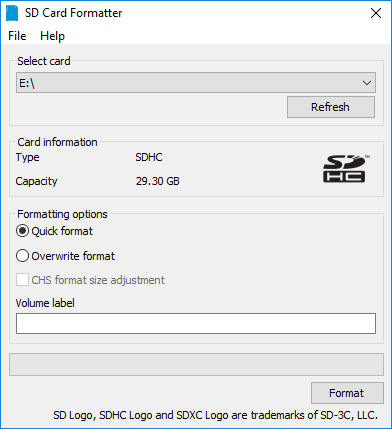
\includegraphics{Images/Jetson_Nano-Getting_Started-Windows-SD_Card_Formatter.png}
			\caption{SD Memory Card Formatter Dialogue}\label{JetPack:SdFormatierer}
		\end{figure}
		\item Select the correct card drive.
		\item Choose the "Quick Format" option.
		\item Leave the "Volume Label" field unchanged.
		\item Click the "Format" button. A warning dialogue will appear. Confirm by clicking "Yes."
	\end{itemize}
\end{enumerate}

\subsubsection{Writing the Image File Using Etcher}

Once the microSD card is formatted, the JetPack image file can be written to it using Etcher:

\begin{enumerate}
	\item \textbf{Download and Launch Etcher:}
	Download Etcher from \url{https://www.balena.io/etcher/}. Install and launch the application. The main dialogue, shown in Figure~\ref{JetPack:Etcher}, will appear.
	\begin{figure}[h!]
		\centering
		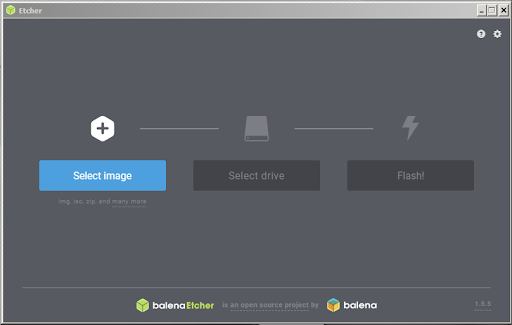
\includegraphics[width=\textwidth]{Images/Jetson_Nano-Getting_Started-Windows-Etcher.png}
		\caption{Etcher Main Dialogue}\label{JetPack:Etcher}
	\end{figure}
	
	\item \textbf{Select the Image File:}
	Click the "Select image" button and choose the downloaded JetPack image file.
	
	\item \textbf{Handle Unformatted Cards:}
	If the microSD card is not formatted, Etcher will display an error, as shown in Figure~\ref{JetPack:NichtFormatiert}. Format the card before proceeding.
	\begin{figure}[h!]
		\centering
		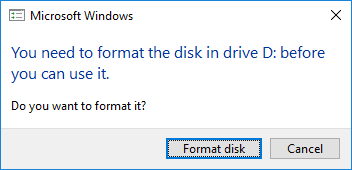
\includegraphics{Images/Jetson_Nano-Getting_Started-Windows-Etcher_Cancel.png}
		\caption{Error Dialogue for Unformatted Card}\label{JetPack:NichtFormatiert}
	\end{figure}
	
	\item \textbf{Start Flashing:}
	Click the "Flash!" button to start writing the image file to the microSD card. The process may take around 10 minutes when using a USB 3.0 interface. After writing, Etcher will validate the image.
	
	\item \textbf{Ignore Windows Warnings:}
	After the process completes, Windows may display a message stating that the microSD card cannot be read, as shown in Figure~\ref{JetPack:NichtLesen}. This message can be ignored. Safely remove the card from the drive.
	\begin{figure}[h!]
		\centering
		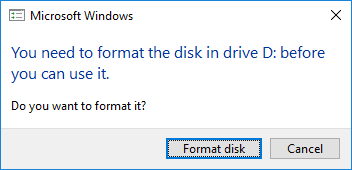
\includegraphics{Images/Jetson_Nano-Getting_Started-Windows-SD_Card_Prompt.png}
		\caption{Windows Message for Unreadable MicroSD Card}\label{JetPack:NichtLesen}
	\end{figure}
\end{enumerate}

\subsubsection{Final Steps}

Once the microSD card is prepared, it can be inserted into the Jetson Nano. On the first boot, the system will guide you through initial configuration steps, including selecting a graphical or headless installation.

This process ensures a smooth setup and prepares the Jetson Nano for further development.




\section{Configuring with a Graphical User Interface and Initial Startup}

With the microSD card containing the JetPack operating system prepared, the Jetson Nano is ready for its initial configuration. At this stage, users must decide between two operational modes:

\begin{itemize}
	\item \textbf{Utilizing a Graphical User Interface (GUI):} Offers a user-friendly, visual interface suitable for most users, especially for those unfamiliar with command-line operations.
	\item \textbf{Operating without a GUI (Headless Mode):} Ideal for resource-constrained environments or when operating the Jetson Nano remotely via SSH.
\end{itemize}

\bigskip

It is important to note that this decision is final during the initial configuration and cannot be changed without reinstalling the operating system. A reinstall would erase all prior settings and require reinstallation of additional software not included in the base OS.

\bigskip

This section outlines the steps for configuring the Jetson Nano with a graphical user interface.

\subsection{Preparation Before Powering On}

Before powering on the Jetson Nano, ensure the following components are correctly connected and ready:

\begin{enumerate}
	\item \textbf{Monitor:} Connect a compatible monitor using an HDMI cable.
	\item \textbf{Keyboard and Mouse:} Attach a standard USB keyboard and mouse for input.
	\item \textbf{Power Supply Unit (PSU):} Use an appropriate power adapter to power the Jetson Nano, but do not connect it yet.
	\item \textbf{MicroSD Card:} Insert the prepared microSD card into the designated slot on the Jetson Nano.
\end{enumerate}

\subsection{Powering On and Initial Setup}

After connecting the peripherals and inserting the microSD card, follow these steps to power on and configure the Jetson Nano:

\begin{enumerate}
	\item \textbf{Power on the Monitor:} Ensure the monitor is switched on before starting the Jetson Nano.
	\item \textbf{Connect the Power Supply:} Plug the power adapter into the Jetson Nano. This will automatically power on the device.
	\item \textbf{System Boot:} The green PWR LED on the Jetson Nano will light up, indicating that the system is booting. The boot process may take several minutes, depending on the speed of the microSD card and the system configuration.
	\item \textbf{Configuration Screen:} Once the boot sequence is complete, the system will display the initial configuration screen. Follow the on-screen prompts to:
	\begin{itemize}
		\item Set up language and region preferences.
		\item Create a user account with a username and password.
		\item Configure network settings (Wi-Fi or Ethernet).
		\item Adjust display resolution and other graphical settings, if necessary.
	\end{itemize}
\end{enumerate}

\subsection{Conclusion}

Upon completing the configuration, the Jetson Nano will load the graphical desktop environment, making it ready for development and use. The GUI provides an accessible and intuitive interface for managing files, running applications, and performing various development tasks. The initial setup ensures that the system is tailored to the user's requirements, providing a seamless experience moving forward.



\subsection{First Start}

The initial boot process of the Jetson Nano requires configuring several essential settings. Follow the steps below to ensure a successful setup:

\begin{itemize}
	\item \textbf{End User License Agreement (EULA):} The first screen presents NVIDIA's EULA for the Jetson Nano software. Read and accept the agreement to proceed.
	
	\item \textbf{Language and Keyboard Preferences:} Select your preferred language and configure the keyboard layout to match the connected keyboard. These settings ensure accurate input and interface language.
	
	\item \textbf{Time Zone Configuration:} Choose the appropriate time zone based on your geographic location to ensure correct timekeeping and system scheduling.
	
	\item \textbf{User Account Configuration:} During the initial setup, the system will prompt you to create a user account. For consistency and ease of access, the following recommendations can be used:
	\begin{itemize}
		\item \textbf{Name:} \texttt{MSR-Lab}
		\item \textbf{Computer Name:} \texttt{JetsonNanoMSRLab}
		\item \textbf{User Name:} \texttt{msrjetson}
		\item \textbf{Password:} \texttt{MSR}
		\item \textbf{Login Type:} \texttt{Automatic Login}
	\end{itemize}
	Using automatic login ensures the system boots directly into the desktop environment without requiring a password, which is particularly useful for standalone or embedded applications.
	
	\item \textbf{Partition Size:} The final step involves specifying the partition size for the system. For standard applications, it is recommended to allocate the maximum partition size to utilize the full capacity of the microSD card effectively.
\end{itemize}

Once these settings are completed, the system will finalize the setup and prepare the operating environment. The Jetson Nano will then reboot and load the configured environment, ready for development and operation.




\subsection{After Logging In}

Upon successful configuration, the Jetson Nano will display a welcoming message, as shown in Figure~\ref{Jetson:Willkommen}. This indicates that the setup process has been completed, and the system is now ready for use.

\begin{figure}[h!]
	\centering
	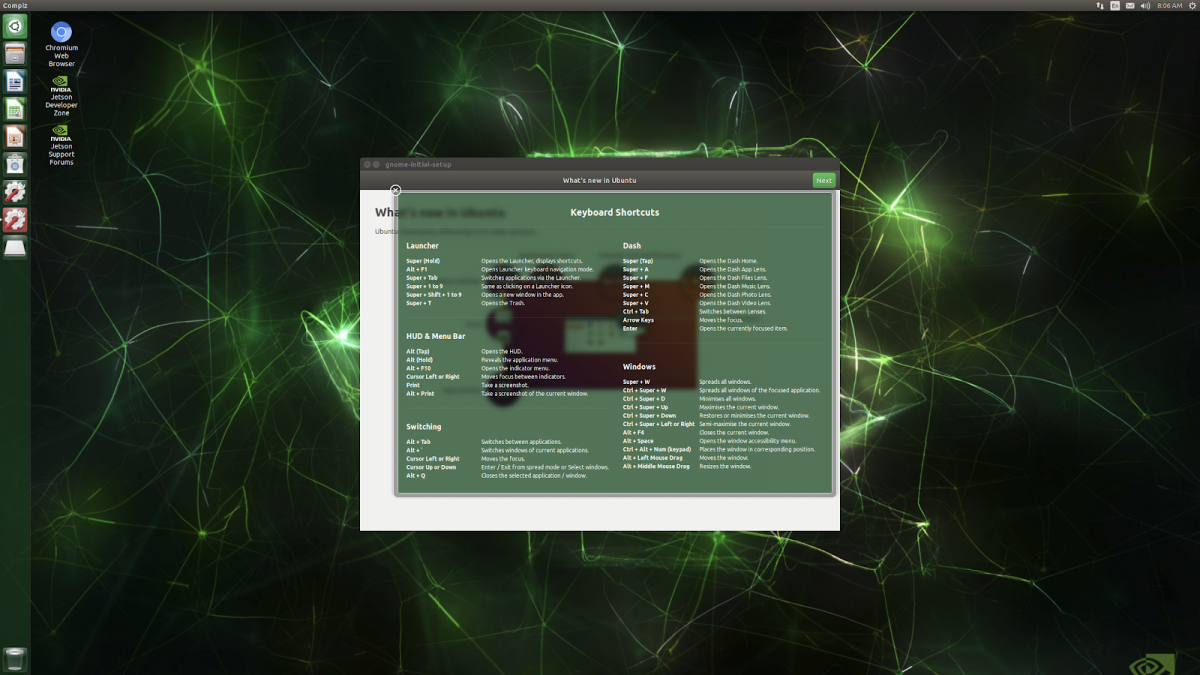
\includegraphics[width=\textwidth]{Images/Jetson_Nano-Getting_Started-Setup_Welcome_Screen.png}
	\caption{Welcome message displayed after the initial setup of Jetson Nano.}
	\label{Jetson:Willkommen}
\end{figure}

\section{Setup Without Graphical Interface}

In edge computing scenarios, the Jetson Nano is often deployed without the ability to connect a monitor or keyboard. This section outlines the process for setting up the Jetson Nano to operate without a graphical interface, suitable for headless configurations.

\subsection{Required Components}
To perform the setup without a graphical interface, you will need the following components:
\begin{itemize}
	\item A microSD card preloaded with the operating system.
	\item Jetson Nano development board.
	\item 5V power supply with a barrel jack connector.
	\item Ethernet cable for internet access.
	\item USB cable with a microUSB connector for data transfer.
	\item A personal computer (PC) for configuration.
	\item An Ethernet connector or network port on the PC.
\end{itemize}

\subsection{Configuration Process}
Since the Jetson Nano lacks a direct visual interface in this setup, it must be connected to a PC for configuration. Follow these steps to ensure a successful setup:

\begin{enumerate}
	\item \textbf{Connect the Power Supply:} Use a 5V power supply with a barrel jack connector to power the Jetson Nano. However, do not connect it yet.
	\item \textbf{Connect to the PC:} Establish a connection between the Jetson Nano and the PC using a microUSB cable. This will enable data transfer and basic communication.
	\item \textbf{Establish an Internet Connection:} Connect an Ethernet cable from the Jetson Nano to a network port or router to provide internet access.
	\item \textbf{Insert the microSD Card:} Insert the microSD card containing the preloaded operating system into the Jetson Nano.
	\item \textbf{Power On the Jetson Nano:} Plug in the power supply. The Jetson Nano will boot up and verify its configuration.
\end{enumerate}

\subsection{Important Note:}
\begin{itemize}
	\item Do not connect a monitor to the Jetson Nano during the setup process. The absence of a monitor signals the system to configure itself for operation without a graphical user interface.
	\item If a monitor is connected, the Jetson Nano will default to installing and configuring a graphical interface, which may not be desired in headless setups.
\end{itemize}

By following the steps above, the Jetson Nano will boot into a headless mode, ready for further configuration via remote access tools like SSH.



\section{Remote Access to the Jetson Nano}

The Jetson Nano can be configured and accessed remotely, eliminating the need for a direct connection to a monitor or keyboard. This section explains how to establish a remote connection from Linux, macOS, or Windows systems.

\subsection{Access via Linux or macOS}

After powering on the Jetson Nano, the connected USB device will be listed under the \texttt{/dev} directory on the host system. For instance, it might appear as \texttt{tty.usbmodemFD133}. A terminal emulator, such as \texttt{screen}, can be used to establish a connection:

\begin{verbatim}
	screen /dev/tty.usbmodemFD133 115200
\end{verbatim}

This command opens a terminal session to communicate with the Jetson Nano. Ensure you have the necessary permissions to access the USB device.

\subsection{Access via Windows}

On a Windows system, the Jetson Nano's interface will appear as a COM port. You can use the \texttt{putty} application to establish a connection via the serial interface. In the \texttt{putty} configuration window:
\begin{enumerate}
	\item Select \textbf{Serial} as the connection type.
	\item Specify the COM port (e.g., \texttt{COM3}) detected by Windows.
	\item Set the baud rate to \texttt{115200}.
	\item Click \textbf{Open} to start the session.
\end{enumerate}

\subsection{Configuration of the Jetson Nano}

Once the connection is established, the Jetson Nano's installation wizard, \texttt{oem-config}, will guide you through the configuration process. This includes:
\begin{enumerate}
	\item Accepting the NVIDIA End User License Agreement (EULA) for the Jetson Nano software.
	\item Setting the language and keyboard layout to match your region and input device.
	\item Selecting the appropriate time zone.
	\item Defining the following system settings:
	\begin{itemize}
		\item \textbf{System Name:} \texttt{MSR-Lab}
		\item \textbf{Computer Name:} \texttt{JetsonNanoMSRLab}
		\item \textbf{User Name:} \texttt{msrjetson}
		\item \textbf{Password:} \texttt{MSR}
		\item \textbf{Login Type:} Automatic Login
	\end{itemize}
\end{enumerate}

\subsection{SSH Access to the Jetson Nano}

After completing the configuration, the Jetson Nano can be accessed remotely using SSH or \texttt{putty}. For instance, on Linux or macOS, open a terminal and use the following command:

\begin{verbatim}
	ssh msrjetson@JetsonNanoMSRLab
\end{verbatim}

Replace \texttt{JetsonNanoMSRLab} with the actual hostname or IP address of the Jetson Nano if it has been updated. This provides secure shell access for remote management and further configuration.




\section{Switching on and Activating Secure Shell (SSH)}

Secure Shell (\ac{ssh}) allows remote access to the Jetson Nano, making it possible to operate the device without a keyboard, mouse, or monitor. The only requirement is that the Jetson Nano is connected to a network via Ethernet or WLAN.

\subsection{Installation of SSH}

The Jetson Nano's operating system includes \ac{ssh} by default, so no additional installation is necessary. However, it needs to be activated to enable its use.

\subsection{Activation of SSH}

To activate \ac{ssh}, the \ac{ssh} server must be started using the following command:

\medskip

\SHELL{sudo /etc/init.d/ssh start}

\medskip

Since this command must be executed each time \ac{ssh} is used, it is recommended to automate the process with the following command:

\medskip

\SHELL{sudo update-rc.d ssh defaults}

\medskip

This ensures that \ac{ssh} is permanently available, even after a system reboot. Alternatively, you can create an empty file named \texttt{ssh} in the root directory. If this file exists, \ac{ssh} is automatically enabled upon the next boot.

\bigskip

For another activation method, access the system settings via the following command:

\medskip

\SHELL{sudo raspi-config}

\medskip

In the configuration dialog, navigate to \texttt{Start Menu > Settings > Configuration}, switch to the \texttt{Interfaces} tab, and set the \texttt{SSH} option to \texttt{Enabled}. Confirm the changes and restart the Jetson Nano with:

\medskip

\SHELL{sudo reboot}

\subsection{Access via User Name and IP Address}

To access the Jetson Nano via \ac{ssh}, you need the user name and password configured during the initial setup, as well as the device's IP address. The IP address can be identified using the following command:

\medskip

\SHELL{ifconfig}

\medskip

This command will display the current network settings, including the IP address.

\subsection{SSH Client on Windows}

Since 2017, Windows has included an \ac{ssh} implementation based on OpenSSH, integrated into the PowerShell command line. To establish an \ac{ssh} connection:

\begin{enumerate}
	\item Open PowerShell from the Start menu.
	\item Enter the following command, replacing \texttt{username} with the Jetson Nano's user name and \texttt{<IPAdresseDesJetsonNanos>} with the device's IP address:
	
	\medskip
	
	\SHELL{ssh username@<IPAdresseDesJetsonNanos>}
	
	\medskip
	
	\item When connecting for the first time, confirm the Jetson Nano's \ac{ssh} keys by typing \texttt{yes}.
	\item Enter the password for the Jetson Nano user account to complete the connection.
\end{enumerate}

With these steps, remote access to the Jetson Nano is established, allowing for management and configuration tasks to be performed efficiently.





\section{Remote Desktop}

When operating the Jetson Nano without peripherals like a monitor, keyboard, or mouse, remote desktop access becomes essential. A lightweight and efficient remote desktop access server, \SHELL{xrdp}, can be utilized for this purpose. 

\subsection{Installation of XRDP}

The installation of \SHELL{xrdp} on the Jetson Nano is straightforward. Execute the following command in the terminal:

\medskip

\SHELL{sudo apt-get install xrdp}

\medskip

After the installation completes, restart the Jetson Nano to apply the changes. Once the system reboots, verify the successful installation of \SHELL{xrdp} using the \SHELL{nmap} command on the host PC:

\medskip

\SHELL{nmap jetson}

\medskip

The output should confirm that the \SHELL{xrdp} service is active, as shown:

\begin{verbatim}
	Starting Nmap 7.70 ( https://nmap.org ) at 2019-04-13 01:39 BST
	Nmap scan report for jetson (192.168.1.118)
	Host is up (0.0025s latency).
	Not shown: 996 closed ports
	PORT     STATE SERVICE
	22/tcp   open  ssh
	111/tcp  open  rpcbind
	3389/tcp open  ms-wbt-server
	Nmap done: 1 IP address (1 host up) scanned in 1.25 seconds
\end{verbatim}

\subsection{Using Remote Desktop Protocol (RDP)}

Remote Desktop Protocol (RDP) is proprietary, but Microsoft provides a free Remote Desktop Viewer for most platforms. To connect via RDP:

\begin{enumerate}
	\item Install the Microsoft Remote Desktop application on the host computer.
	\item Open the application and select \glqq Add Desktop\grqq{} to configure the Jetson Nano connection.
	\item Enter the IP address of the Jetson Nano and configure settings such as resolution for optimal usability.
\end{enumerate}

Once connected, the session can run in full-screen mode or within a resizable window.

\subsection{Behavior of the RDP Desktop}

The desktop displayed through RDP differs slightly from the physical desktop. Instead of the default Unity-style L4T interface, a standard Ubuntu desktop with Gnome is used. Notably:

\begin{itemize}
	\item The RDP desktop is persistent until the user explicitly logs off. Closing the RDP window does not terminate the session.
	\item Simultaneous login to both the physical desktop and the RDP session is not supported.
\end{itemize}

\subsection{Power Settings for Wireless Connections}

For users accessing the Jetson Nano over a wireless network, ensure that the Wi-Fi does not turn off to save power. To configure this:

\begin{itemize}
	\item Open the \glqq Settings\grqq{} menu in the Gnome application.
	\item Navigate to the \glqq Power\grqq{} section.
	\item Disable the option \glqq Turn off Wi-Fi to save power\grqq{}.
\end{itemize}

After this setup, peripherals like the monitor, keyboard, and mouse can be unplugged, as they are no longer necessary for operation.

\section{Conclusion}

In conclusion, the implementation of a remote desktop solution on the Jetson Nano significantly enhances its usability in headless configurations. With the integration of advanced deep learning frameworks such as TensorFlow, the license plate detection system achieves real-time accuracy and efficiency, meeting the demands of modern edge computing applications.
